\documentclass[12pt, a4paper]{article}

%%%%%%%%%%%%%%%紙張大小設定%%%%%%%%%%%%%%%
% \paperwidth=65cm
% \paperheight=160cm

%%%%%%%%%%%%%%%引入Package%%%%%%%%%%%%%%%
\usepackage[margin=1cm]{geometry} % 上下左右距離邊緣2cm
\usepackage{mathtools,amsthm,amssymb} % 引入 AMS 數學環境
\usepackage{yhmath}      % math symbol
\usepackage{graphicx}    % 圖形插入用
\usepackage{fontspec}    % 加這個就可以設定字體
\usepackage{type1cm}	 % 設定fontsize用
\usepackage{titlesec}   % 設定section等的字體
\usepackage{titling}    % 加強 title 功能
\usepackage{fancyhdr}   % 頁首頁尾
\usepackage{tabularx}   % 加強版 table
\usepackage[square, comma, numbers, super, sort&compress]{natbib}
% cite加強版
\usepackage[unicode, pdfborder={0 0 0}, bookmarksdepth=-1]{hyperref}
% ref加強版
\usepackage[usenames, dvipsnames]{color}  % 可以使用顏色
\usepackage[shortlabels, inline]{enumitem}  % 加強版enumerate
\usepackage{xpatch}

\graphicspath{ {images/} }
% \usepackage{tabto}      % tab
% \usepackage{soul}       % highlight
% \usepackage{ulem}       % 字加裝飾
\usepackage{wrapfig}     % 文繞圖
%\usepackage{lipsum}
% \usepackage{floatflt}    % 浮動 figure
\usepackage{float}       % 浮動環境
% \usepackage{caption}    % caption 增強
% \usepackage{subcaption}    % subfigures
% \usepackage{setspace}    % 控制空行
% \usepackage{mdframed}   % 可以加文字方框
% \usepackage{multicol}   % 多欄
% \usepackage[abbreviations]{siunitx} % SI unit
% \usepackage{dsfont}     % more mathbb

%%%%%%%%%%%%%%%%%%%TikZ%%%%%%%%%%%%%%%%%%%%%%
% \usepackage{tikz}
% \usepackage{circuitikz}

%%%%%%%%%%%%%%中文 Environment%%%%%%%%%%%%%%%
\usepackage[CheckSingle, CJKmath]{xeCJK}  % xelatex 中文
\usepackage{CJKulem}	% 中文字裝飾
\setCJKmainfont{Source Han Sans}
% 設定中文為系統上的字型,而英文不去更動,使用原TeX字型

% \XeTeXlinebreaklocale "zh"             %這兩行一定要加,中文才能自動換行
% \XeTeXlinebreakskip = 0pt plus 1pt     %這兩行一定要加,中文才能自動換行

%%%%%%%%%%%%%%%字體大小設定%%%%%%%%%%%%%%%
% \def\normalsize{\fontsize{10}{15}\selectfont}
% \def\large{\fontsize{40}{60}\selectfont}
% \def\Large{\fontsize{50}{75}\selectfont}
% \def\LARGE{\fontsize{90}{20}\selectfont}
% \def\huge{\fontsize{34}{51}\selectfont}
% \def\Huge{\fontsize{38}{57}\selectfont}

%%%%%%%%%%%%%%%Theme Input%%%%%%%%%%%%%%%%
% \input{themes/chapter/neat}
% \input{themes/env/problist}

%%%%%%%%%%%titlesec settings%%%%%%%%%%%%%%
% \titleformat{\chapter}{\bf\Huge}
            % {\arabic{section}}{0em}{}
% \titleformat{\section}{\centering\Large}
            % {\arabic{section}}{0em}{}
% \titleformat{\subsection}{\large}
            % {\arabic{subsection}}{0em}{}
% \titleformat{\subsubsection}{\bf\normalsize}
            % {\arabic{subsubsection}}{0em}{}
% \titleformat{command}[shape]{format}{label}
            % {編號與標題距離}{before}[after]

%%%%%%%%%%%%variable settings%%%%%%%%%%%%%%
% \numberwithin{equation}{section}
% \setcounter{secnumdepth}{4}  %章節標號深度
% \setcounter{tocdepth}{1}  %目錄深度
% \setcounter{section}{0}  %section 起始 counter
% \graphicspath{{images/}}  % 搜尋圖片目錄

%%%%%%%%%%%%%%%頁面設定%%%%%%%%%%%%%%%
\newcolumntype{C}[1]{>{\centering\arraybackslash}p{#1}}
\setlength{\headheight}{15pt}  %with titling
\setlength{\droptitle}{-2cm} %title 與上緣的間距
% \posttitle{\par\end{center}} % title 與內文的間距
\parindent=12pt %設定縮排的距離
% \parskip=1ex  %設定行距
% \pagestyle{empty}  % empty: 無頁碼
% \pagestyle{fancy}  % fancy: fancyhdr

% use with fancygdr
% \lhead{\leftmark}
% \chead{}
% \rhead{}
% \lfoot{}
% \cfoot{}
% \rfoot{\thepage}
% \renewcommand{\headrulewidth}{0.4pt}
% \renewcommand{\footrulewidth}{0.4pt}

% \fancypagestyle{firststyle}
% {
  % \fancyhf{}
  % \fancyfoot[C]{\footnotesize Page \thepage\ of \pageref{LastPage}}
  % \renewcommand{\headrule}{\rule{\textwidth}{\headrulewidth}}
% }

%%%%%%%%%%%%%%%重定義一些command%%%%%%%%%%%%%%%
\renewcommand{\contentsname}{目錄}  %設定目錄的標題名稱
\renewcommand{\refname}{參考資料}  %設定參考資料的標題名稱
\renewcommand{\abstractname}{\LARGE Abstract} %設定摘要的標題名稱

%%%%%%%%%%%%%%%特殊功能函數符號設定%%%%%%%%%%%%%%%
\DeclarePairedDelimiter{\abs}{\lvert}{\rvert}
\DeclarePairedDelimiter{\norm}{\lVert}{\rVert}
\DeclarePairedDelimiter{\inpd}{\langle}{\rangle} % inner product
\DeclarePairedDelimiter{\ceil}{\lceil}{\rceil}
\DeclarePairedDelimiter{\floor}{\lfloor}{\rfloor}
\DeclareMathOperator{\adj}{adj}
\DeclareMathOperator{\sech}{sech}
\DeclareMathOperator{\csch}{csch}
\DeclareMathOperator{\arcsec}{arcsec}
\DeclareMathOperator{\arccot}{arccot}
\DeclareMathOperator{\arccsc}{arccsc}
\DeclareMathOperator{\arccosh}{arccosh}
\DeclareMathOperator{\arcsinh}{arcsinh}
\DeclareMathOperator{\arctanh}{arctanh}
\DeclareMathOperator{\arcsech}{arcsech}
\DeclareMathOperator{\arccsch}{arccsch}
\DeclareMathOperator{\arccoth}{arccoth}
\newcommand{\np}[1]{\\[{#1}] \indent}
\newcommand{\transpose}[1]{{#1}^\mathrm{T}}
%%%% Geometry Symbol %%%%
\newcommand{\degree}{^\circ}
\newcommand{\Arc}[1]{\wideparen{{#1}}}
\newcommand{\Line}[1]{\overleftrightarrow{{#1}}}
\newcommand{\Ray}[1]{\overrightarrow{{#1}}}
\newcommand{\Segment}[1]{\overline{{#1}}}

%%%%%%%%%%%%%%%證明、結論、定義等等的環境%%%%%%%%%%%%%%%
\renewcommand{\proofname}{\bf 證明:} %修改Proof 標頭
\newtheoremstyle{mystyle}% 自定義Style
  {6pt}{15pt}%       上下間距
  {}%               內文字體
  {}%               縮排
  {\bf}%            標頭字體
  {.}%              標頭後標點
  {1em}%            內文與標頭距離
  {}%               Theorem head spec (can be left empty, meaning 'normal')

% 改用粗體,預設 remark style 是斜體
\theoremstyle{mystyle}	% 定理環境Style
\newtheorem{theorem}{定理}
\newtheorem{definition}{定義}
\newtheorem{formula}{公式}
\newtheorem{condition}{條件}
\newtheorem{supposition}{假設}
\newtheorem{conclusion}{結論}
\newtheorem{corollary}{推論}
\newtheorem{lemma}{引理}
\newtheorem{property}{性質}

\titlespacing*{\section} {0pt}{0ex}{0ex}

%%%%%%%%%%%%%%%Title%%%%%%%%%%%%%%%
\title{MLDS 2017 Spring HW1 - Language Model}
\author{B03901056 孫凡耕 B03901070 羅啓心\\
        B03901032 郭子生 B03901003 許晉嘉}
\date{\vspace{-5ex}}

\begin{document}
\maketitle 
\thispagestyle{empty}
\section{Environment}
\begin{enumerate}
  \item 硬體資訊: 
    \begin{tabular}{|C{4cm}|C{3cm}|C{3cm}|C{3cm}|}
      \hline
      OS & CPU & GPU & Memory \\
      \hline
      \texttt{Arch linux 4.10} & \texttt{i7 3.4 GHz} &
      \texttt{GTX 1070}  & \texttt{32 GB}  \\
      \hline
    \end{tabular}
  \item 所使用的 \texttt{python} library:
    \begin{tabular}{|c|c|}
      \hline
      \texttt{spacy 1.6.0} & \texttt{nltk 3.2.2} \\
      \hline
    \end{tabular}
\end{enumerate}
% End of Environment

\section{Model description}
% End of Model description

\section{Improvement}
\begin{enumerate}
  \item 僅使用 Training Data 中,長度在特定範圍之內的句子\\
    特短的句子,大多屬於雜訊或是較無意義的短句(e.g. somebody said,);
    特長的句子,也均爲雜訊居多,若納入特長的句子亦會使 training model
    維度過高,造成記憶體空間不足。且特短及特長的句子,
    本身在 Training Data 中所佔的比例也不高(如 Figure 1.)。
    \begin{figure}[!htb]
      \centering
      \minipage{0.32\textwidth}
       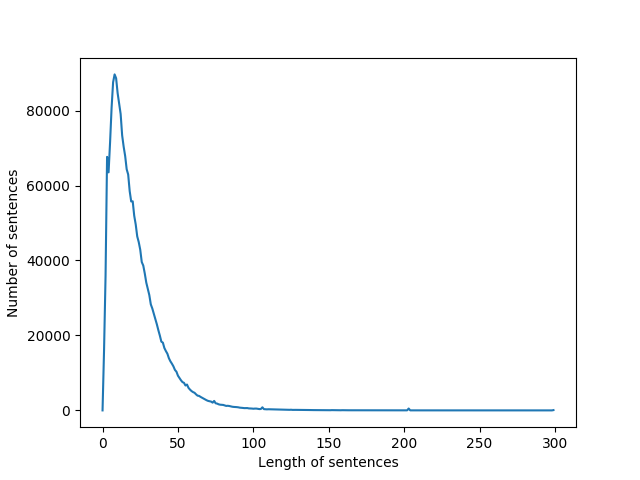
\includegraphics[scale=0.37]{sent_len_dis.png}
       \caption{句子長度分佈}
      \endminipage\hfill
      \minipage{0.32\textwidth}
        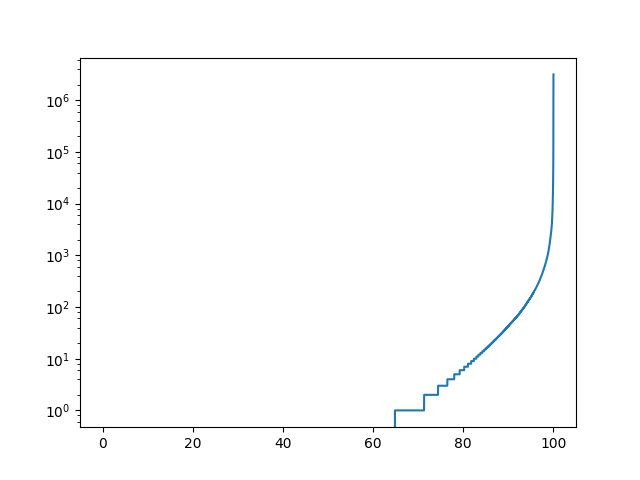
\includegraphics[scale=0.37]{word_dis2.png}
        \caption{單字出現次數分佈}
      \endminipage\hfill
      \minipage{0.32\textwidth}
        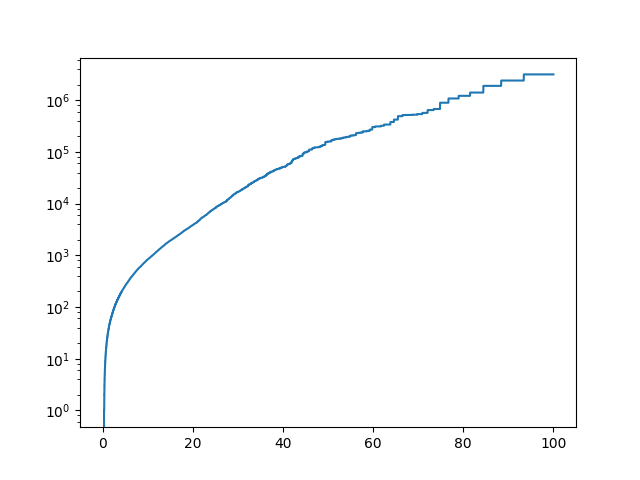
\includegraphics[scale=0.37]{word_dis.png}
        \caption{單字出現次數比例分佈}
      \endminipage
    \end{figure}
  \item 將出現次數過少的單字從 corpus 中移除\\
    原本 corpus 的字量過大,會造成記憶體空間不足以及訓練困難,因此,將在
    Training Data 中出現次數較少的單字移除(視爲 unknown word),可使
    訓練學習的過程加速。從上圖 Figure 2 可看出七成左右的單字不在 pretrained
    corpus 內或是出現次數少於兩次,而從 Figure 3 可看出這些單字又僅佔不到
    總單字量的一個百分點,因此,將其刪除對於訓練的過程有較大的助益。
  \item 將 Training Data 中,開頭及結尾的部分刪去\\
    由於 Training Data 中幾乎所有文章,開頭及結尾皆相當於目錄或版權資訊等,
    較不爲一般常用語的句子。有利訓練過程的進行。
  \item Dependency Tree\\
    Dependency tree 可表示句子當中各單字之間的關聯。因此,將資料轉爲
    dependency tree 後,可更爲有效的分出每個句子中各個合法的語句,使訓練
    的資料更爲廣泛且一般。
\end{enumerate}
% End of Improvement

\section{Experiment}
% End of Experiment

\section{Team division}
\begin{table}[h]
\centering
\begin{tabular}{ |C{2cm}|C{10cm}| }
  \hline
  孫凡耕 & \\
  \hline
  羅啓心 & \\
  \hline
  郭子生 & \\
  \hline
  許晉嘉 & 資料處理、撰寫報告\\
  \hline
\end{tabular}
\end{table}
% End of Team division

\end{document}
